\begin{enumerate}
%1
\item \textbf{รูปแบบไม่กำหนด (Indeterminate form)}
รูปแบบไม่กำหนดมีทั้งหมด 7 รูปแบบด้วยกัน ได้แก่
\begin{figure}[h!]
\centering
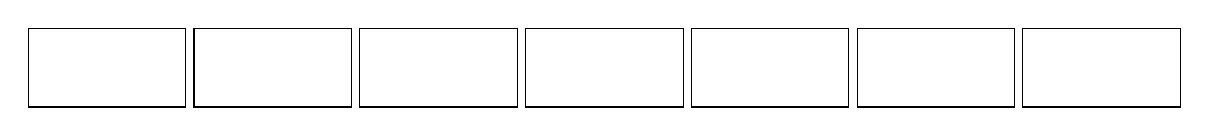
\begin{tikzpicture}
\foreach \x in {1,...,7}
\draw[xshift = 3*\x] (2*\x,0) rectangle (2*\x+2,1);
\end{tikzpicture}
\end{figure}

จงหาว่าลิมิตต่อไปนี้เป็นรูปแบบไม่กำหนดหรือไม่ ถ้าใช่ให้คำนวณลิมิตโดยใช้กฎของโลปิตาล

\begin{tasks}[after-skip = 120pt, after-item-skip = 120pt](3)
\task $\lim_{x \rightarrow 1} \frac{x^4-1}{x-1}$
\task $\lim_{x \rightarrow 0} \frac{x^4-1}{x-1}$
\task $\lim_{x \rightarrow 2} \frac{x^3-8}{x^2-x-2}$
\task $\lim_{x \rightarrow 0} \frac{\sin (3x)}{x}$
\task $\lim_{x \rightarrow 0} \frac{e^x}{\sin x}$
\task $\lim_{x \rightarrow +\infty} \frac{\ln x}{x}$
\end{tasks}

\item \textbf{การหาปริพันธ์โดยใช้นิยาม}

จงเติมประโยคต่อไปนี้ให้ถูกต้อง (ข้อมูลที่จำเป็นทั้งหมดสามารถหาได้ในโจทย์แล้ว ไม่จำเป็นต้องหาอนุพันธ์ด้วยตัวเอง)

\begin{tasks}(1)
\task ถ้า $\dx x^2 = 2x$ แล้ว $\int 2x\,dx = \blank$
\task ถ้า $\dx \blank = 3\cos(3x)$ แล้ว $\int 3 \cos(3x) \, dx = \sin (3x) + C$
\task ถ้า $\dx (x+1)^4 = \blank$ แล้ว $\int 4(x+1)^3 \, dx = \blank$
\task ถ้า $\dx\blank = \blank $ แล้ว $\int (xe^x+x) \, dx = xe^x + C$
\task ถ้า $\dx x^4 = 4x^3$ จะได้ว่า $\dx \frac{1}{4}x^4 = \blank$ ฉะนั้น $\int x^3 \,dx = \blank + C$
\end{tasks}

\newpage
\item \textbf{การหาปริพันธ์โดยใช้สูตรพื้นฐาน}

จงหาปริพันธ์ต่อไปนี้ โดยแสดงวิธีทำทุกขั้นตอน
\begin{tasks}[after-skip = 100pt, after-item-skip = 100pt](3)
\task $\int 9 \, dx$
\task $\int -2 \, dx$
\task $\int x^3 \, dx$
\task $\int x^5 \, dx$
\task $\int x^{5/2} \, dx$
\task $\int \frac{1}{\sqrt{x}} \, dx$
\task $\int \frac{1}{3x^4} \, dx$
\task $\int (x^4 - x^3) \, dx$
\task $\int (x^6 + 1) \, dx$
\task $\int (6x^5 + 6x^2) \, dx$
\task $\int \left(3x + \frac{4}{x^2}\right) \, dx$
\task $\int (x+1)(x+2) \, dx$
\task $\int \frac{2x^3+3x^2}{2} \, dx$
\task $\int \frac{x^2-3x+2}{2x-2} \, dx$
\task $\int (x+1)^3 \, dx$
\end{tasks}

\end{enumerate}

\end{document}